% !TeX root = main.tex
% !TEX program = pdflatex

\chapter{Adquisición de Datos (DAQ)}\label{cap:daq}


Una vez acondicionada la señal analógica, el siguiente paso es su digitalización. El sistema de adquisición de datos (DAQ) es el encargado de realizar la discretización de la señal tanto en el tiempo (muestreo) como en la amplitud (cuantificación). En este capítulo analizaremos las arquitecturas de los convertidores A/D, los errores intrínsecos al proceso de conversión y los criterios de diseño para garantizar la integridad de la información en el dominio digital.


\section{Muestreo y Retención (Sample and Hold)}\label{sec:muestreo}

El proceso de digitalización comienza con el muestreo. Para que un convertidor A/D pueda procesar una señal que varía continuamente, es necesario \emph{congelar} su valor durante el tiempo que dura la conversión. El bloque \emph{Sample and Hold (S\&H)} actúa como una memoria analógica que captura el valor instantáneo de la señal y lo mantiene estable. 

\paragraph{Arquitectura Básica del S\&H}
El circuito fundamental consta de cuatro elementos críticos, como se detalla en la Figura~\ref{fig:circuito_sh_esquema}:
\begin{enumerate}
    \item \emph{Amplificador de Entrada (Buffer)}: Presenta una impedancia de entrada muy alta para no cargar al sensor o a la etapa de acondicionamiento previa.
    \item \emph{Interruptor Analógico}: Implementado habitualmente mediante transistores MOSFET (puertas de transmisión CMOS). Su resistencia en conducción ($R_{on}$) debe ser mínima.
    \item \emph{Condensador de Retención ($C_h$)}: El elemento que almacena la carga eléctrica proporcional al voltaje de muestra.
    \item \emph{Amplificador de Salida (Buffer)}: Evita que el propio ADC descargue el condensador durante la medida, presentando una impedancia de salida casi nula.
\end{enumerate}

\begin{marginfigure}
    \centering
    \shorthandoff{>}
    \begin{tikzpicture}[american, scale=0.9, font=\scriptsize]
        \ctikzset{amplifiers/fill=blue!5, resistors/scale=0.6, capacitors/scale=0.7}
        
        % Buffers
        \draw (0,2) node[op amp, scale=0.6] (OA1) {};
        \draw (4,2) node[op amp, scale=0.6] (OA2) {};
        
        % Conexiones OA1
        \draw (OA1.+) -- ++(-0.5,0) node[left] {$V_{in}$};
        \draw (OA1.out) -- ++(0,-0.4) -| (OA1.-);
        
        % Interruptor
        \draw (OA1.out) to[cspst, l=SW, *-*] ++(1.5,0) coordinate (nodeC);
        
        % Condensador Ch
        \draw (nodeC) to[C, l=$C_h$, *-] ++(0,-1.2) node[ground] {};
        
        % Conexión OA2
        \draw (nodeC) -- (OA2.+);
        \draw (OA2.out) -- ++(0,-0.4) -| (OA2.-);
        \draw (OA2.out) to[short, -o] ++(0.5,0) node[right] {$V_{out}$};
        
        % Control lógico
        \draw[dashed, ->, >=stealth] (1.3, 3) node[above] {Control} -- (1.3, 2.2);

    \end{tikzpicture}
    \caption[Esquema circuital de un S\&H.]{Configuración clásica de un circuito de muestreo y retención. El uso de dos seguidores de tensión garantiza el aislamiento de la carga almacenada en $C_h$. El interruptor SW es una puerta de transmisión CMOS. El amplificador de salida evita que el propio ADC descargue el condensador durante la medida.}\label{fig:circuito_sh_esquema}
\end{marginfigure}

\paragraph{Dinámica del Muestreo: Tiempo de Adquisición}
Cuando el interruptor se cierra (fase de \textit{Sample}), el condensador se carga a través de la resistencia $R_{on}$. Este proceso sigue una dinámica de primer orden con una constante de tiempo $\tau = R_{on} \cdot C_h$.

Se define el \emph{Tiempo de Adquisición} ($t_{acq}$) como el tiempo necesario para que el voltaje en $C_h$ alcance el valor de entrada con un error menor a $1/2$ LSB. Para un ADC de $n$ bits, se requiere:
\begin{equation}\label{eq:tacq}
    t_{acq} > \tau \cdot \ln(2^{n+1}) \approx \tau \cdot 0,7 \cdot (n+1)
\end{equation}

\marginnote{\textbf{Compromiso de diseño en $C_h$:} 
    Si $C_h$ es muy \emph{grande}, el tiempo de adquisición es lento. Si $C_h$ es muy \emph{pequeño}, las corrientes de fuga descargarán el condensador demasiado rápido durante la fase de retención.
}

\paragraph{Imperfecciones en la Fase de Retención (\textit{Hold})}
Una vez abierto el interruptor, el circuito debería mantener $V_{out}$ constante, pero aparecen dos errores sistemáticos críticos:
\begin{itemize}
    \item \emph{Droop Rate} (Tasa de caída): Debido a la corriente de polarización del operacional de salida y a las fugas del interruptor ($I_{leak}$), el condensador se descarga lentamente. La deriva de tensión se calcula como:
    \begin{equation}
        \frac{dV}{dt} = \frac{I_{leak}}{C_h}
    \end{equation}
    \item \emph{Feedthrough} (Acoplamiento): Una parte de la señal de entrada puede "filtrarse" a la salida a través de la capacidad parásita del interruptor abierto, degradando el aislamiento.
\end{itemize}

\begin{marginfigure}
    \centering
    \shorthandoff{>}
    \begin{tikzpicture}
        \begin{axis}[
            width=\linewidth, height=5cm,
            xlabel={Tiempo}, ylabel={Voltaje},
            xmin=0, xmax=5, ymin=0, ymax=1.5,
            axis lines=left, xtick=\empty, ytick=\empty,
            font=\scriptsize
        ]
            % Escalón ideal
            \draw[gray, dashed] (axis cs:1, 0.5) -- (axis cs:1, 1.2) -- (axis cs:4, 1.2);
            % Droop real
            \addplot[thick, blue, domain=1:4] {1.2 - 0.05*(x-1)};
            % Anotación Droop
            \draw[<->, red] (axis cs:3.8, 1.2) -- (axis cs:3.8, 1.06) node[midway, right] {Droop};
            
            \node[blue] at (axis cs:2.5, 1.3) {Fase de Retención};
        \end{axis}
    \end{tikzpicture}
    \caption{Efecto de la tasa de caída (\textit{droop}) durante la fase de retención. Este error limita el tiempo máximo que el ADC puede tardar en convertir sin perder precisión.}\label{fig:droop_effect}
\end{marginfigure}

\paragraph{Incertidumbre Temporal: Aperture Jitter}
Como se muestra en la Figura~\ref{fig:jitter_error}, el instante exacto en el que el interruptor se abre no es constante debido al ruido en el reloj de muestreo. Esta variación ($\Delta t_a$) produce un error de amplitud que depende de la velocidad de variación de la señal. 

Para que este error sea inferior a un escalón de cuantificación ($Q$), la frecuencia máxima de la señal está limitada por:
\begin{equation}
    f_{max} \leq \frac{1}{2\pi \cdot \Delta t_a \cdot 2^n}
\end{equation}

\marginnote{\textbf{Ejemplo de Ingeniería:}
    Para muestrear una señal de audio de \qty{20}{kHz} con un ADC de \qty{16}{bits}, el jitter del reloj debe ser inferior a \qty{120}{ps}. Esto explica por qué el diseño del \textit{layout} del reloj es crítico en PCBs de alta fidelidad.
}

\begin{marginfigure}
    \centering
    \shorthandoff{>}
    \begin{tikzpicture}[scale=0.9, font=\scriptsize]
        \begin{axis}[
            width=\linewidth, height=5cm,
            axis lines=left, xlabel={$t$}, ylabel={$V$},
            xmin=0, xmax=2, ymin=0, ymax=2,
            xtick=\empty, ytick=\empty
        ]
            % Señal rápida
            \addplot[thick, gray, domain=0.5:1.5] {x+0.2};
            
            % Jitter
            \draw[red, thick, <->] (axis cs:0.9, 0.5) -- (axis cs:1.1, 0.5) node[midway, below] {$\Delta t_a$};
            
            % Error resultante
            \draw[blue, thick, <->] (axis cs:1.6, 1.1) -- (axis cs:1.6, 1.3) node[midway, right] {$\Delta V$};
            
            \draw[dashed, gray] (axis cs:0.9, 0) -- (axis cs:0.9, 1.1) -- (axis cs:1.6, 1.1);
            \draw[dashed, gray] (axis cs:1.1, 0) -- (axis cs:1.1, 1.3) -- (axis cs:1.6, 1.3);
        \end{axis}
    \end{tikzpicture}
    \caption{Relación entre el jitter temporal ($\Delta t_a$) y el error de amplitud ($\Delta V$). A mayor pendiente de la señal, más crítico es el ruido de fase del reloj.}\label{fig:jitter_error}
\end{marginfigure}

%figura de un circuito S\&H
% \begin{marginfigure}
%     \centering
%     \shorthandoff{>}
%     \begin{tikzpicture}[scale=1]
%         % Componentes del S&H
%         \draw[thick] (0,0) node[left] {$V_{in}$} to[short, o-] (1,0) to[R, l=$R_{on}$] (1,-2) to[short] (0,-2) node[left] {GND};
%         \draw[thick] (1,0) to[C, l=$C_{hold}$] (3,0) to[short, -o] (4,0) node[right] {$V_{hold}$};
%         \draw[thick] (3,0) to[short] (3,-2) node[below] {GND};
%         \node at (2,-1) {S\&H};
%     \end{tikzpicture}
%     \caption[Esquema de un circuito Muestreo y Retención.]{Esquema simplificado de un circuito S\&H. El interruptor controla el muestreo de la señal de entrada $V_{in}$ y el capacitor $C_{hold}$ mantiene el valor durante la conversión.}\label{fig:sh_circuito}
% \end{marginfigure}

\paragraph{Teorema de Nyquist y Aliasing}
Como se introdujo en el Capítulo 5, para evitar la pérdida de información, la frecuencia de muestreo $f_s$ debe ser estrictamente superior al doble de la frecuencia máxima de la señal $f_{max}$. Si no se cumple esta condición, las componentes de alta frecuencia se solapan en la banda base, un fenómeno irreversible conocido como \emph{aliasing}.

% ejemplo de aliasing con una señal de 1 kHz muestreada a 1.5 kHz y de no aliasing con la misma señal muestreada a 3 kHz. caption explicativa de porque la informacón se pierde en el primer caso y se conserva en el segundo.
% \begin{marginfigure}
%     \centering    
%     \begin{tikzpicture}[scale=1]
%         \pgfkeys{/pgf/number format/.cd, use comma=false} % asegurar punto decimal
%         \begin{axis}[
%             width=\linewidth, height=5cm,
%             xlabel={Tiempo}, ylabel={$V_{in}$},
%             xmin=0, xmax=10, ymin=-1.2, ymax=1.5,
%             axis lines=left, xtick=\empty, ytick=\empty,
%             font=\scriptsize
%         ]
%             % Señal de 1 kHz
%             \addplot[thick, gray!50, domain=0:10, samples=100] {sin(deg(2*pi*1*x))};
%             \node[gray] at (axis cs:2, 1.2) {Señal Original (1 kHz)};

%             % Muestreo a 1.5 kHz (aliasing)
%             \draw[red, thick] (axis cs:0.6667,-0.8660) -- (axis cs:1.3333,-0.8660);
%             \draw[red, thick] (axis cs:1.3333,0.8660) -- (axis cs:2,0.8660);
%             \draw[red, thick] (axis cs:2,0) -- (axis cs:2.6667,0);
%             \draw[red, thick] (axis cs:2.6667,-0.8660) -- (axis cs:3.3333,-0.8660);
%             \draw[red, thick] (axis cs:3.3333,0.8660) -- (axis cs:4,0.8660);
%             \draw[red, dashed] (axis cs:0.6667,0) -- (axis cs:0.6667,-0.8660);
%             \fill[red] (axis cs:0.6667,-0.8660) circle (1.5pt);
%             \draw[red, dashed] (axis cs:1.3333,0) -- (axis cs:1.3333,0.8660);
%             \fill[red] (axis cs:1.3333,0.8660) circle (1.5pt);
%             \draw[red, dashed] (axis cs:2,0) -- (axis cs:2,0);
%             \fill[red] (axis cs:2,0) circle (1.5pt);
%             \draw[red, dashed] (axis cs:2.6667,0) -- (axis cs:2.6667,-0.8660);
%             \fill[red] (axis cs:2.6667,-0.8660) circle (1.5pt);
%             \draw[red, dashed] (axis cs:3.3333,0) -- (axis cs:3.3333,0.8660);
%             \fill[red] (axis cs:3.3333,0.8660) circle (1.5pt);
%             \draw[red, dashed] (axis cs:4,0) -- (axis cs:4,0);
%             \fill[red] (axis cs:4,0) circle (1.5pt);
%             \node[red] at (axis cs:4.5, -0.8) {Muestreo a 1.5 kHz (Aliasing)};

%             % Muestreo a 3 kHz (no aliasing)
%             \draw[blue, thick] (axis cs:0.3333,0.8660) -- (axis cs:0.6667,0.8660);
%             \draw[blue, thick] (axis cs:0.6667,-0.8660) -- (axis cs:1,-0.8660);
%             \draw[blue, thick] (axis cs:1,0) -- (axis cs:1.3333,0);
%             \draw[blue, thick] (axis cs:1.3333,0.8660) -- (axis cs:1.6667,0.8660);
%             \foreach \x/\y in {0.3333/0.8660, 0.6667/-0.8660, 1/0, 1.3333/0.8660, 1.6667/-0.8660} {
%                 \draw[blue, dashed] (axis cs:\x,0) -- (axis cs:\x,\y);
%                 \fill[blue] (axis cs:\x,\y) circle (1.5pt);
%             }
%             \node[blue] at (axis cs:4.5, -1.1) {Muestreo a 3 kHz (No Aliasing)};
%         \end{axis}
%     \end{tikzpicture}
%     \caption[Ejemplo de Aliasing.]{Comparativa entre muestreo con aliasing (rojo) y sin aliasing (azul) de una señal de 1 kHz. En el primer caso, la frecuencia de muestreo es insuficiente, lo que provoca que la señal digital resultante no represente fielmente la señal original, mientras que en el segundo caso, el muestreo cumple con el criterio de Nyquist, preservando la integridad de la información.}\label{fig:aliasing_ejemplo}
% \end{marginfigure}


% \begin{marginfigure}[2em]
%     \centering
%     \shorthandoff{>}
%     \begin{tikzpicture}[scale=1]
%         \begin{axis}[
%             width=\linewidth, height=5cm,
%             xlabel={Tiempo}, ylabel={$V_{in}$},
%             xmin=0, xmax=10, ymin=-1.2, ymax=1.5,
%             axis lines=left, xtick=\empty, ytick=\empty,
%             font=\scriptsize
%         ]
%             % Señal Analógica
%             \addplot[thick, gray!50, domain=0:10, samples=100] {sin(deg(x))};
%             \node[gray] at (axis cs:2, 1.2) {Analógica};

%             % Muestras (S&H)
%             \foreach \x in {1,2,3,4,5,6,7,8,9} {
%                 \pgfmathsetmacro{\y}{sin(deg(\x))}
%                 \draw[blue, thick] (\x, \y) -- (\x+1, \y);
%                 \draw[blue, dashed] (\x, 0) -- (\x, \y);
%                 \fill[blue] (\x, \y) circle (1.5pt);
%             }
%         \end{axis}
%     \end{tikzpicture}
%     \caption[Proceso de Muestreo y Retención.]{Acción del circuito S\&H. El sistema captura el valor instantáneo (muestreo) y lo mantiene constante (retención) para que el ADC realice la aproximación sucesiva sin errores por variación de entrada.}\label{fig:muestreo_sh}
% \end{marginfigure}

\paragraph{Error de Apertura y Jitter}
El S\&H ideal es instantáneo, pero los circuitos reales sufren limitaciones temporales. 
\begin{itemize}
    \item \emph{Tiempo de apertura}: Es el tiempo que tarda el interruptor interno en abrirse completamente. Durante este intervalo, la señal sigue variando, introduciendo una incertidumbre en el valor capturado.
    \item \emph{Jitter de apertura}: Es la variación aleatoria del instante de muestreo debido al ruido en el reloj de sincronismo. En señales de alta frecuencia, una pequeña variación en el tiempo ($\Delta t$) se traduce en un error masivo en tensión ($\Delta V$), como se deduce de:
    \begin{equation}
        \Delta V = \frac{dV(t)}{dt} \cdot \Delta t
    \end{equation}
\end{itemize}

\marginnote{\textbf{Criterio de Diseño:} Para no perder resolución, el error por jitter debe ser menor que la mitad de un escalón de cuantificación ($1/2$ LSB). Esto impone exigencias de estabilidad extremas a los osciladores de cuarzo en sistemas de audio de alta fidelidad.}

\section{Cuantificación: El Límite en Amplitud}\label{sec:cuantificacion}

La cuantificación es el proceso de asignar un valor numérico discreto a la muestra analógica retenida. Este proceso introduce inherentemente un error, ya que existe una pérdida de información al mapear un rango continuo en un número finito de niveles.

\paragraph{Resolución y LSB}
Un convertidor de $n$ bits dispone de $2^n$ niveles de salida. El salto mínimo de tensión detectable se denomina \emph{escalón de cuantificación} o \emph{Peso del Bit Menos Significativo} (LSB):
\begin{equation}
    Q = V_{LSB} = \frac{V_{FS}}{2^n}
\end{equation}
donde $V_{FS}$ es el rango de fondo de escala (\textit{Full Scale}).

\begin{marginfigure}[2em]
    \centering
    \shorthandoff{>}
    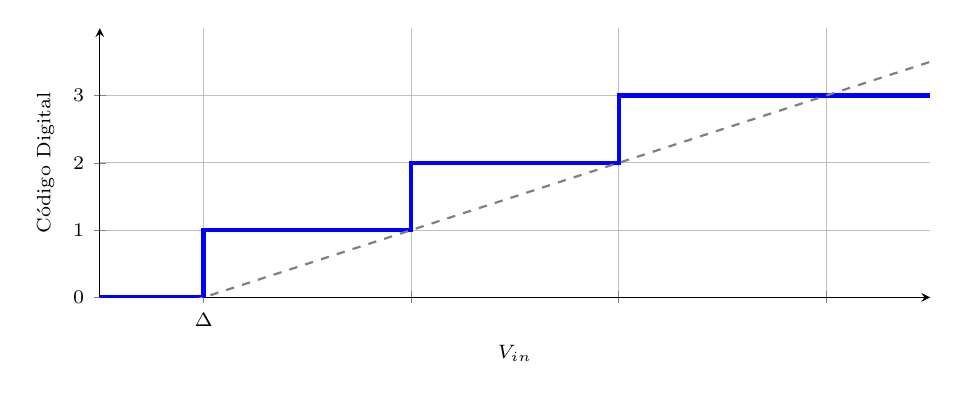
\begin{tikzpicture}
        \begin{axis}[
            width=\linewidth, height=5cm,
            xlabel={$V_{in}$}, ylabel={Código Digital},
            xmin=0, xmax=4, ymin=0, ymax=4,
            axis lines=left,
            xtick={0.5, 1.5, 2.5, 3.5}, xticklabels={$\Delta$},
            ytick={0,1,2,3},
            grid=both, font=\scriptsize
        ]
            % Escalera de cuantificación
            \addplot[ultra thick, blue, no marks] coordinates {(0,0) (0.5,0) (0.5,1) (1.5,1) (1.5,2) (2.5,2) (2.5,3) (3.5,3) (4,3)};
            % Línea ideal
            \addplot[thick, gray, dashed, domain=0:4] {x - 0.5};
        \end{axis}
    \end{tikzpicture}
    \caption[Función de transferencia de un ADC.]{Función de transferencia ideal de un cuantificador. La característica de "escalera" muestra cómo múltiples valores de entrada mapean al mismo código digital, originando el error de cuantificación.}\label{fig:escalera_cuant}
\end{marginfigure}

\paragraph{Ruido de Cuantificación}
El error de cuantificación $\epsilon_q$ oscila entre $\pm Q/2$. Si la señal es compleja y cubre muchos niveles, este error se modela como un ruido blanco con distribución uniforme. Su valor eficaz (RMS) es:
\begin{equation}
    V_{q,RMS} = \frac{Q}{\sqrt{12}}
\end{equation}

A partir de este valor, se deduce la relación señal-ruido teórica máxima para un ADC ideal de $n$ bits:
\begin{equation}
    \text{SNR}_{max} \approx 6,02 \cdot n + 1,76 \text{ dB}
\end{equation}

\marginnote{\textbf{La Regla de los 6 dB:} Por cada bit adicional que añadimos a nuestro convertidor, mejoramos la relación señal-ruido en aproximadamente \qty{6}{dB} (un factor de 2 en amplitud).}

\section{Arquitecturas de Convertidores A/D}\label{sec:arquitecturas_adc}

No existe el ADC perfecto; la elección de la arquitectura depende del compromiso entre velocidad de muestreo y resolución en bits.

\paragraph{ADC de Aproximaciones Sucesivas (SAR)}
Es el estándar para propósito general y el que integran la mayoría de microcontroladores. Utiliza una estrategia de búsqueda binaria mediante un DAC interno y un comparador. 
\begin{itemize}
    \item \emph{Ventajas:} Buen equilibrio velocidad/consumo/precio.
    \item \emph{Limitación:} Requiere un S\&H externo o integrado y su resolución suele estancarse en los \qty{16}{bits}.
\end{itemize}

\paragraph{ADC Sigma-Delta ($\Sigma\Delta$)}
Es la arquitectura reina en instrumentación de precisión (balanzas, termometría). Se basa en el sobremuestreo masivo y el filtrado digital (conformado de ruido).
\begin{itemize}
    \item \emph{Ventajas:} Resoluciones altísimas (hasta \qty{24}{bits}).
    \item \emph{Limitación:} Muy lento comparado con otras arquitecturas.
\end{itemize}

\paragraph{ADC de Doble Rampa (Integración)}
Es la arquitectura utilizada en los multímetros digitales de banco. Su principio de funcionamiento cancela ruidos periódicos.
\begin{itemize}
    \item \emph{Ventaja:} Excelente rechazo al ruido de red (\qty{50}{Hz} / \qty{60}{Hz}).
\end{itemize}

\begin{table}[ht]
    \centering
    \small
    \caption{Comparativa de arquitecturas ADC.}\label{tab:comparativa_adc}
    \begin{tabularx}{\linewidth}{l X X X}
        \toprule
        \textbf{Tipo} & \textbf{Velocidad} & \textbf{Resolución} & \textbf{Uso Típico} \\
        \midrule
        Flash & Extrema (\unit{GHz}) & Baja (8 bits) & Osciloscopios, Radar. \\
        SAR & Media (\unit{MHz}) & Media (12-16 bits) & Control industrial. \\
        Sigma-Delta & Baja (\unit{kHz}) & Muy alta (24 bits) & Audio, Pesaje. \\
        Integración & Muy baja (\unit{Hz}) & Alta (20 bits) & Multímetros. \\
        \bottomrule
    \end{tabularx}
\end{table}

\section{Parámetros Reales y ENOB}\label{sec:enob}
En 4º curso, el ingeniero debe saber que un ADC de 16 bits rara vez entrega 16 bits de información útil. El ruido térmico, la no linealidad integral (INL) y la no linealidad diferencial (DNL) degradan el rendimiento. Se define el \textbf{ENOB} (\textit{Effective Number of Bits}):
\begin{equation}
    \text{ENOB} = \frac{\text{SINAD}_{dB} - 1,76}{6,02}
\end{equation}

\marginnote{\textbf{SINAD:} Es la relación entre la señal y la suma de ruido más distorsión. Es el parámetro real que debemos buscar en un \textit{datasheet} para conocer la calidad del componente.}